\chapter{Architettura}
\label{sec:architettura}

\begin{figure}
    \centering
    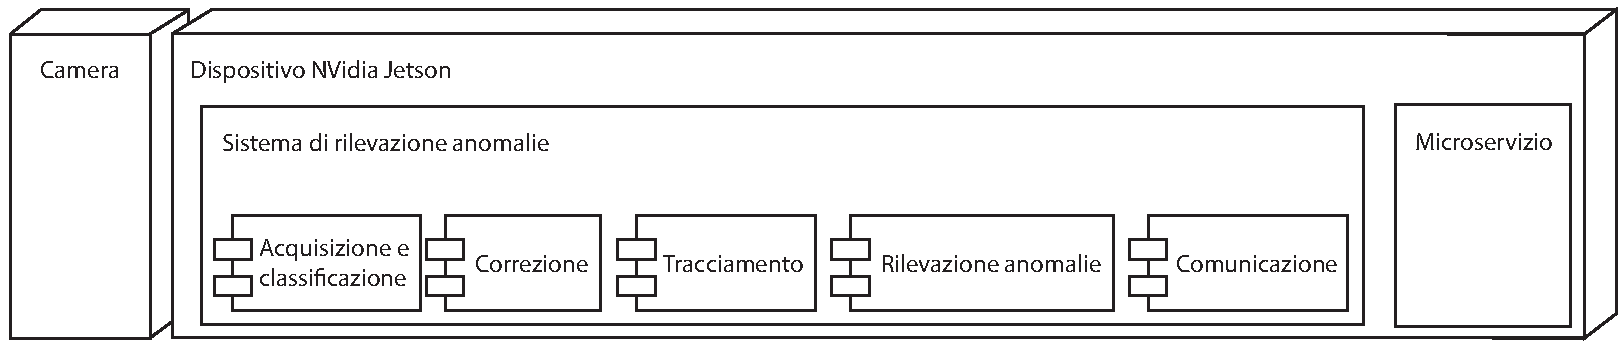
\includegraphics[width=\textwidth]{images/arch.png}
    \caption{Architettura del sistema}
\end{figure}

L'architettura scelta è una pipeline, in quanto l'input del sistema è uno stream video.
Ogni frame dello stream deve essere processato nello stesso modo, e utilizzare una pipeline consente di aggiungere, rimuovere o sostituire moduli, e quindi modificare il processo, in modo semplice e veloce.

Il sistema è implementato sul dispositivo \emph{Nvidia Jetson Xaxier}\cite{arch:jetson} ed è sviluppato su \emph{Ubuntu 18.04}\cite{arch:ubuntu}.
Il linguaggio di sviluppo è \emph{Python 3.6}\cite{arch:python}.
Per la gestione delle operazione di algebra lineare sono stati utilizzati i package \emph{Numpy}\cite{arch:numpy} e \emph{SciPy}\cite{arch:scipy}.
La pipeline di acquisizione è gestita dalla libreria \emph{GStreamer}\cite{arch:gstreamer}.
La classificazione è effettuata dal modulo di inferenza fornito dall'\emph{SDK Nvidia Deepstream}\cite{arch:deepstream}.
Questo modulo di inferenza è configurato per il modello di \emph{Object Detection Scaled--YoloV4}\cite{yolocsp}.
Il tracking è gestito dal tracker \emph{NvDCF} \cite{nvdcf}, anch'esso fornito dall'\emph{SDK Nvidia Deepstream}.
La segnalazione delle anomalie è effettuata utilizzando la libreria \emph{Requests} \cite{arch:requests}.
